\documentclass{article}
\usepackage[utf8]{inputenc}
\usepackage{amsmath,amssymb}
\usepackage{graphicx}
\usepackage{float}
\usepackage{subcaption}
\usepackage{geometry}
\geometry{
    a4paper,
    total={170mm,257mm},
    left=20mm,
    right=20mm,
    top=20mm,
}
\usepackage{listings} % code listings
\lstset{framextopmargin=0pt,frame=lines}
\lstset{
    language=Matlab,
    basicstyle=\footnotesize\ttfamily,
    breaklines=true,
    tabsize=4,
    keepspaces=true,
    columns=flexible,
    % backgroundcolor=\color[gray]{0.9},
    frame=single,
    breaklines=true,%
    morekeywords={matlab2tikz},
    keywordstyle=\color{blue},%
    morekeywords=[2]{1}, keywordstyle=[2]{\color{black}},
    identifierstyle=\color{black},%
    stringstyle=\color{mylilas},
    commentstyle=\color{mygreen},%
    showstringspaces=false,%without this there will be a symbol in the places where there is a space
    numbers=left,
    numberstyle={\tiny \color{black}},% size of the numbers
    numbersep=9pt, % this defines how far the numbers are from the text
    emph=[1]{for,end,break},emphstyle=[1]\color{red}, %some words to emphasise
    %emph=[2]{word1,word2}, emphstyle=[2]{style},
}
\usepackage{color} %red, green, blue, yellow, cyan, magenta, black, white
\definecolor{mygreen}{RGB}{28,172,0} % color values Red, Green, Blue
\definecolor{mylilas}{RGB}{170,55,241}

\title{ENV-541 Sensor Orientation\\Lab 1 - Stochastic Processes}
\author{Michael Spieler}
\date{October 5, 2018}

\begin{document}

\maketitle

\section*{1 Noise realizations plots}

% \begin{figure}[H]
% \centering
% \begin{subfigure}[t]{0.49\textwidth}
% \centering
% 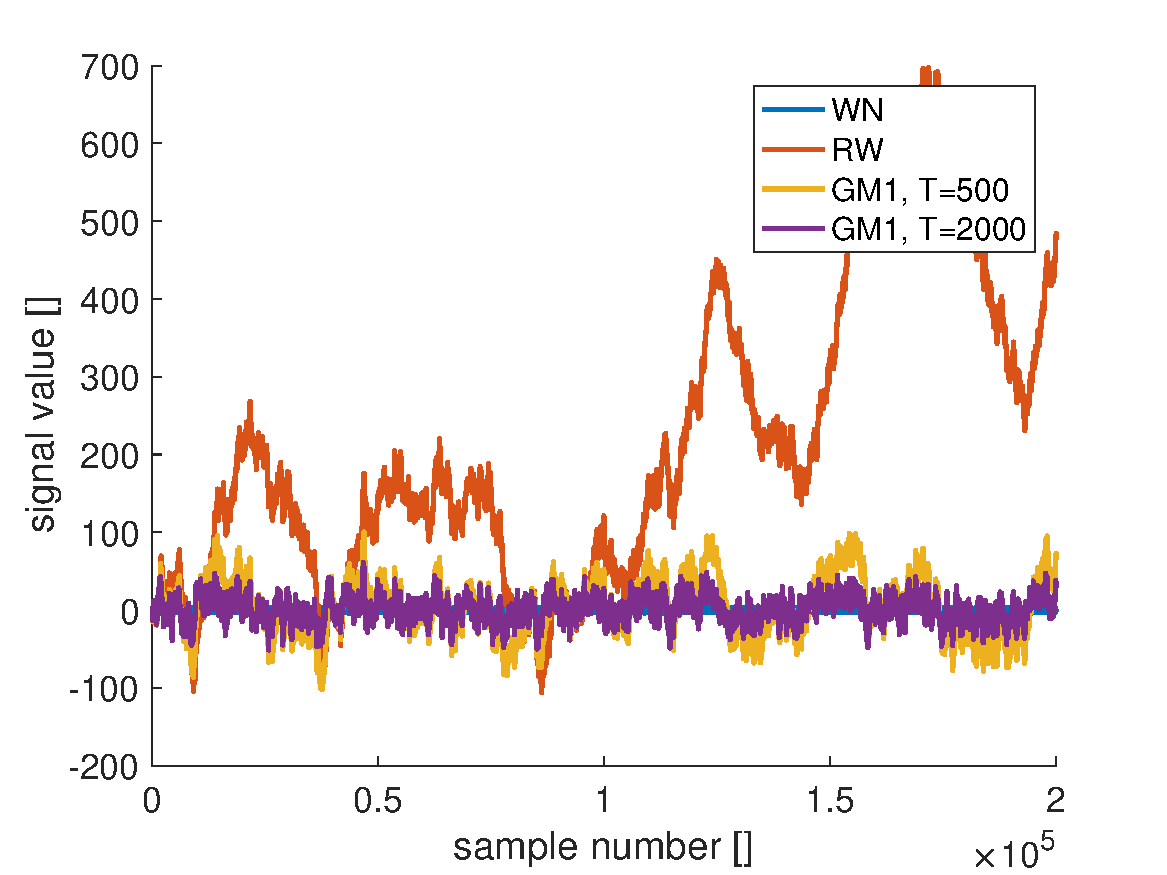
\includegraphics[width=\textwidth]{signal1}
% \end{subfigure}
% ~
% \begin{subfigure}[t]{0.49\textwidth}
% \centering
% 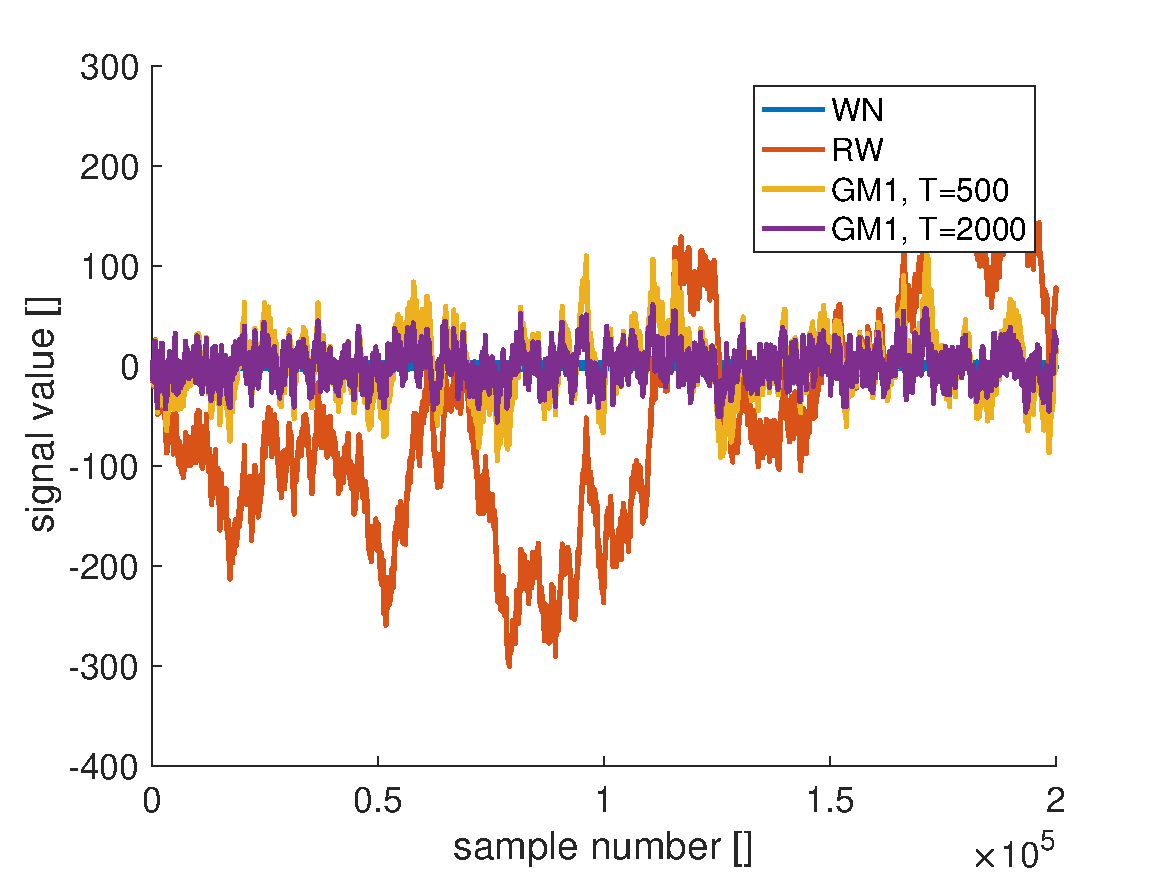
\includegraphics[width=\textwidth]{signal2}
% \end{subfigure}
% ~
% \begin{subfigure}[t]{0.49\textwidth}
% \centering
% 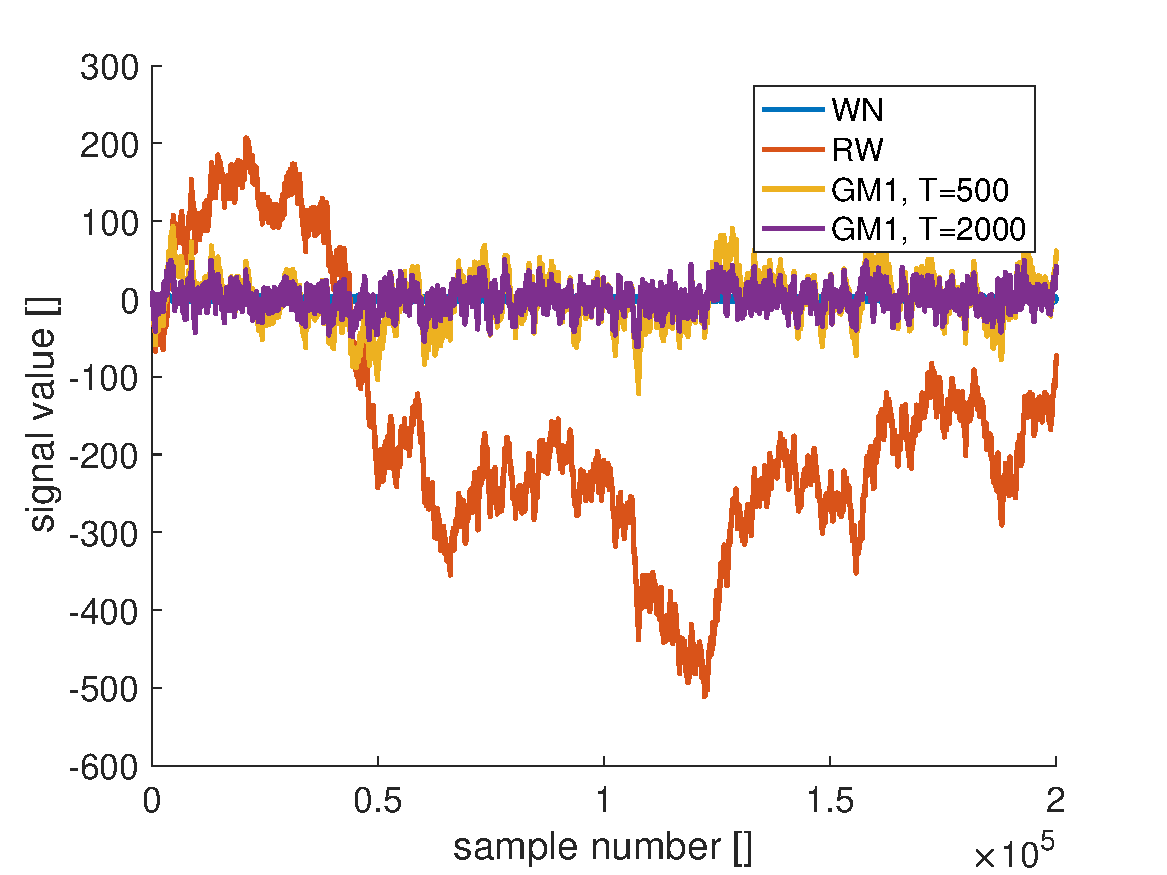
\includegraphics[width=\textwidth]{signal3}
% \end{subfigure}
% \caption{Three different realizations of White Noise (WN), Random Walk (RW) and first order Gauss-Markov (GM1) process with correlation times T=500 and T=2000.}
% \label{fig:signals}
% \end{figure}

\begin{figure}[H]
    \centering
    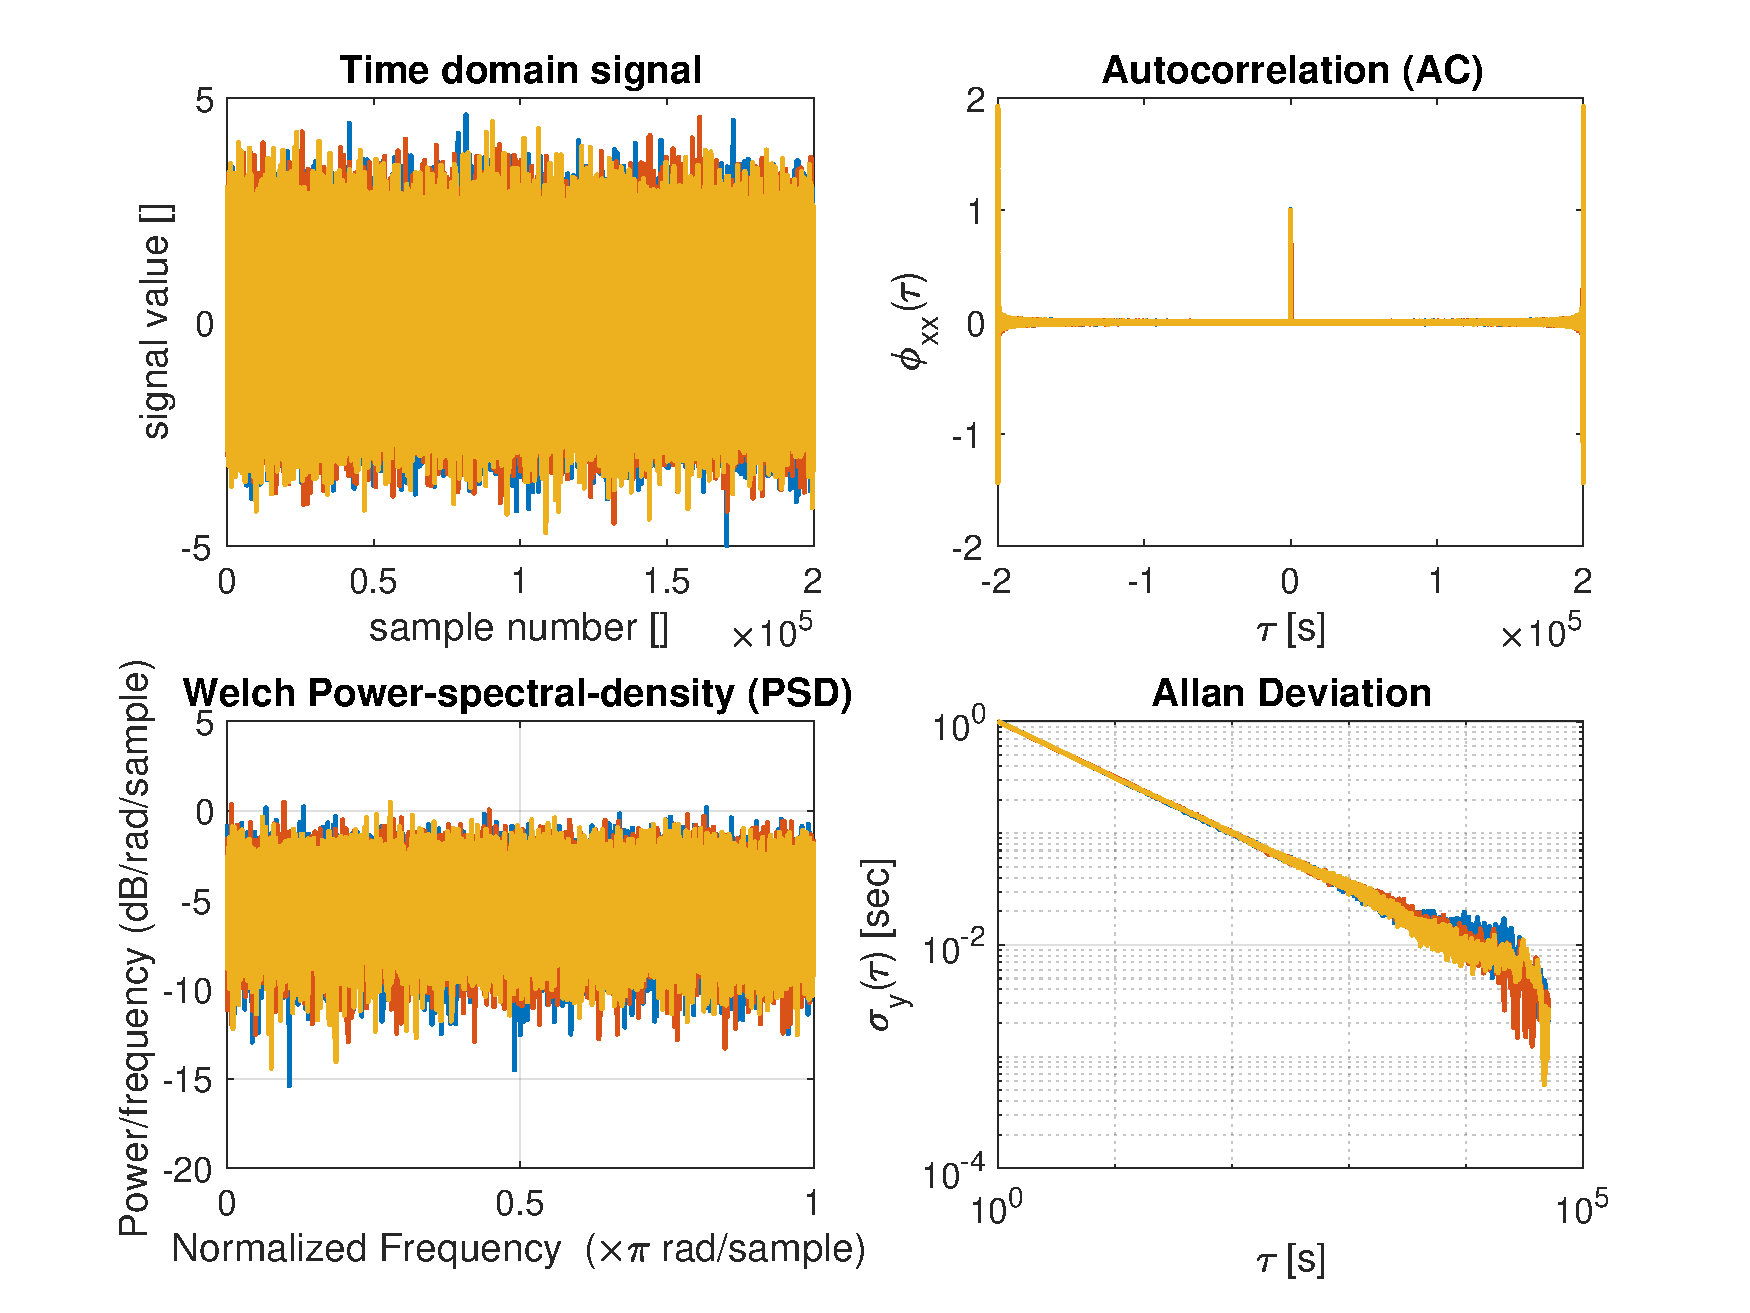
\includegraphics[width=0.9\textwidth]{white_noise}
    \caption{White Noise.}
    \label{fig:white_noise}
\end{figure}

\begin{figure}[H]
    \centering
    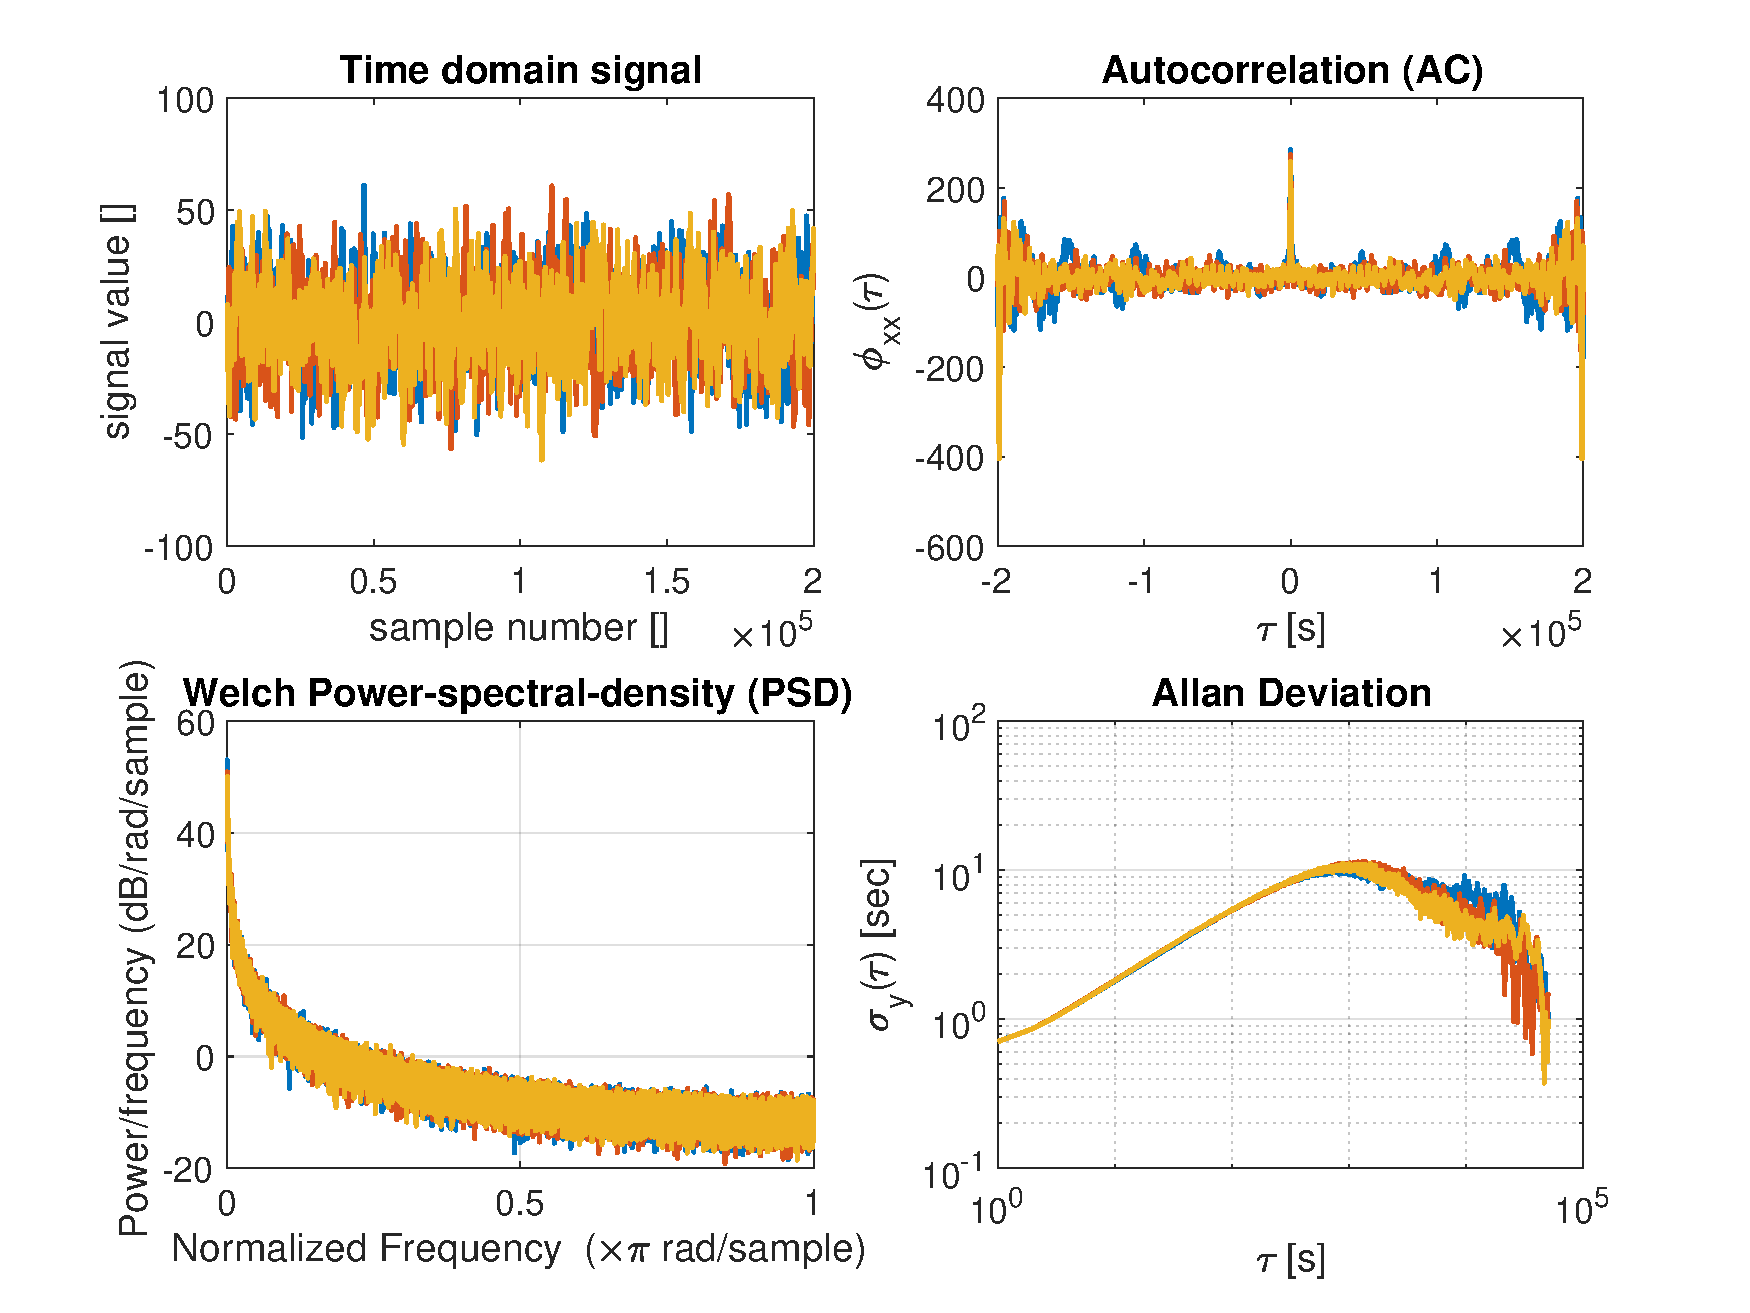
\includegraphics[width=0.9\textwidth]{gm500}
    \caption{first order Gauss-Markov process with correlation time T=500.}
    \label{fig:gm500}
\end{figure}

\begin{figure}[H]
    \centering
    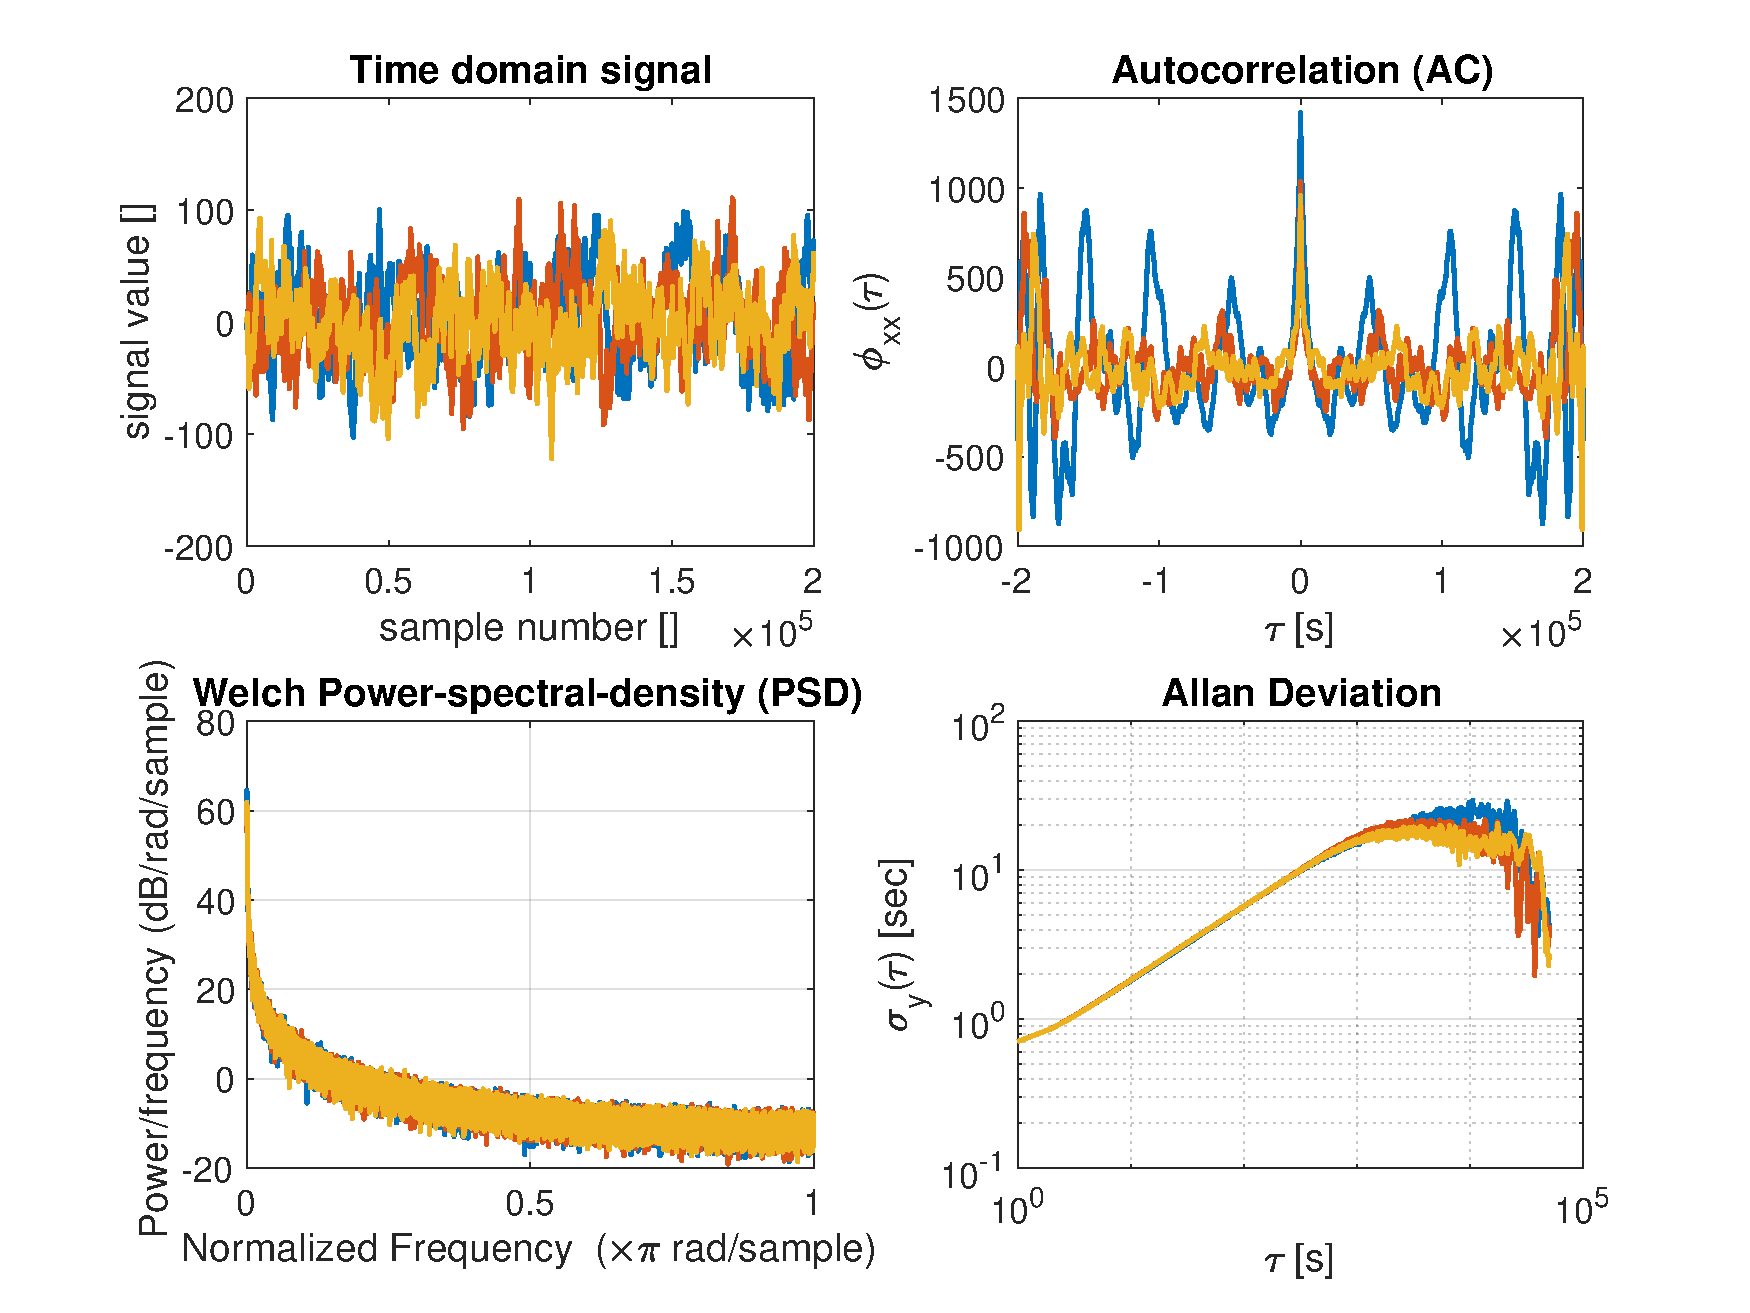
\includegraphics[width=0.9\textwidth]{gm2000}
    \caption{first order Gauss-Markov process with correlation time T=2000.}
    \label{fig:gm2000}
\end{figure}

\begin{figure}[H]
    \centering
    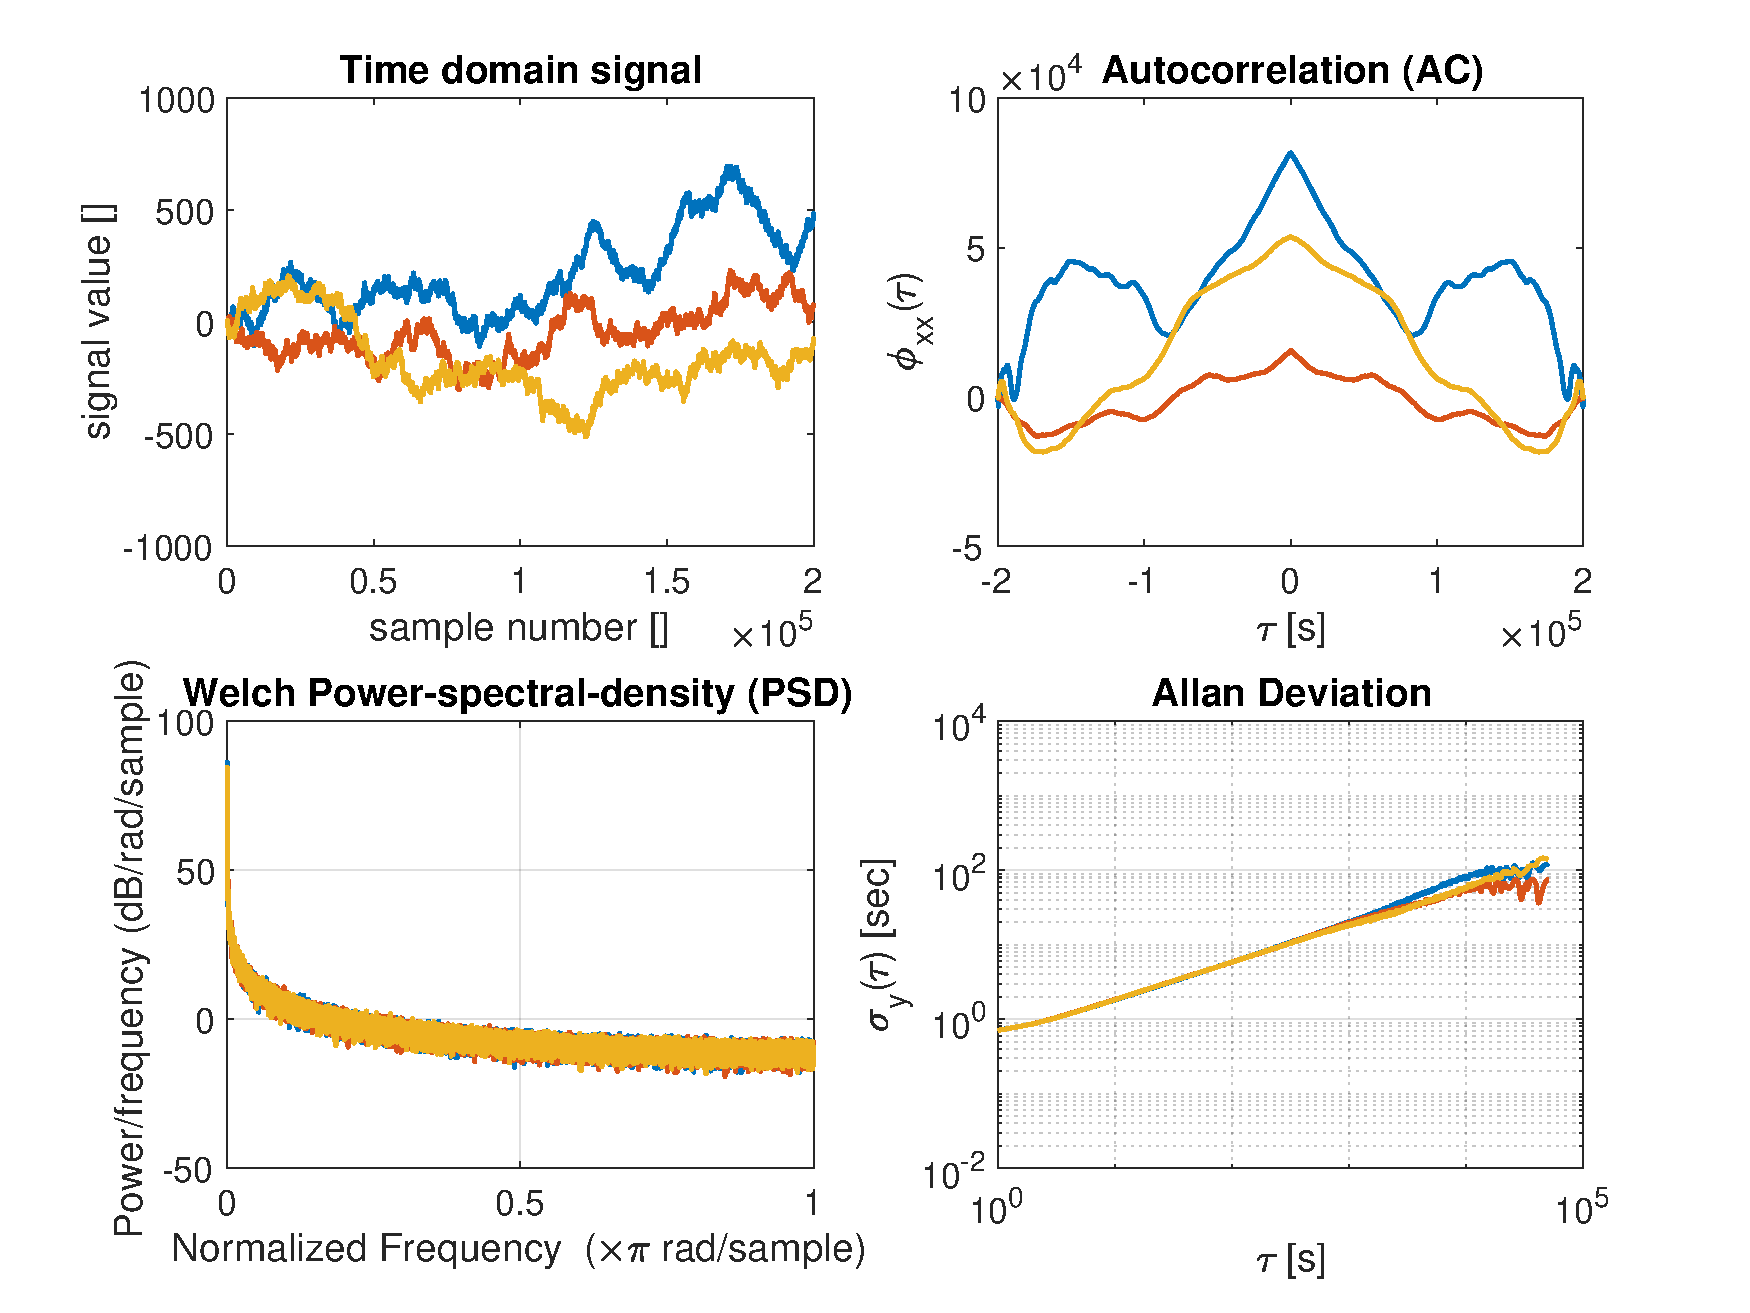
\includegraphics[width=0.9\textwidth]{random_walk}
    \caption{Random Walk.}
    \label{fig:random_walk}
\end{figure}

\section*{2 Analysis}
\subsection*{2.a Autocorrelation function shape}
\begin{description}
    \item[White Noise] The autocorrelation is a dirac.
    \item[1st order Gauss-Markov] Near to the center ($\tau=0$), the autocorrelation resembles an exponentail decay in $\mid\tau\mid$, which is expected. There are lobes further away from $\tau=0$ which does not correspond to the theory but can be explained by the fact that the unbiased version of \verb'xcorr()' was used.
    \item[Random Walk] The autocorrelation should look like a Gauss-Markov with quasi-infinite correlation time (exponential decay in $\tau$), which it does with some imagination.
\end{description}
Note: In both the Gauss-Markov and the random walk sequences the autocorrelation shows weird lobes in the first realization (blue).
Maybe this is due to a badly initialized random number generator since \verb'rng(1)' is used for reproducible plots?

\subsection*{2.b Empirically determined values for standard deviation and correlation length}

Parameter $\beta$ is obtained by reading on the autocorrelation plot the width $T$ of the central peak at $\sigma^2/e$. $\beta = 1/T$

\begin{table}[h]
\centering
\begin{tabular}{llll}
sequence nb. & 1 (blue) & 2 (red) & 3 (orange) \\ \hline
$\sigma^2$ &  1421 & 1034 & 955.6  \\
% $\sigma$ &  37.67 & 32.16 & 30.91  \\
$T$ & 6662 & 3282 & 1838
\end{tabular}
\caption{GMP $T=2000$}
\label{tab:gmp2000}
\end{table}

\begin{table}[h]
\centering
\begin{tabular}{llll}
sequence nb. & 1 (blue) & 2 (red) & 3 (orange) \\ \hline
$\sigma^2$ &  285.1 & 274.6 & 258.8  \\
% $\sigma$ &  16.88 & 16.57 & 16.09  \\
$T$ & 1136 & 1042 & 942
\end{tabular}
\caption{GMP $T=500$}
\label{tab:gmp500}
\end{table}

Tables \ref{tab:gmp500} and \ref{tab:gmp2000} show the measured values for $\sigma^2$ and $T$.
The theoretical values for $\sigma^2$ are $\sigma^2_{GM} = 1/(2\beta)$ with $q=1$ and $\beta=1/T$ which are in this case 1000 and 250 respectively.
The variance $\sigma^2$ is estimated is quite close to the theoreticl value.
However, the values for the correlation length $T$ are off by up to a factor of 3. The reason for the deviation is unclear.

\subsection*{2.c}
The correlation time $T$ characterizes best the underlying process because it depends only on parameter $\beta$.
It tells how close the signal is to white noise.
The smaller $T$, the closer to white noise, the bigger $T$, the closer to a random walk.
% The graphical approach gave better estimates for $\sigma^2$ than for $T$.
% Therefore, the estimated $\sigma^2$ characterizes best the underlying process.
% A $\sigma^2$ close to 1 indicates white noise, while a big $\sigma^2$ indicates a random walk.

\subsection*{2.d}

\begin{table}[h]
\centering
\begin{tabular}{llll}
sequence nb. & 1 & 2 & 3 \\ \hline
$\sigma^2$ & 1.182931e+03 & 9.042480e+02 & 9.889570e+02 \\
$\beta$ & 4.229967e-04 & 5.559729e-04 & 5.066038e-04 \\
$T=1/\beta$ & 2364.1 & 1798.6 & 1973.9
\end{tabular}
\caption{GMP $T=2000$}
\label{tab:fit_gmp2000}
\end{table}

\begin{table}[h]
\centering
\begin{tabular}{llll}
sequence nb. & 1 & 2 & 3 \\ \hline
$\sigma^2$ & 2.664254e+02 & 2.710082e+02 & 2.610238e+02 \\
$\beta$ & 1.880129e-03 & 1.855449e-03 & 1.921333e-03 \\
$T=1/\beta$ & 531.9 & 539.0 & 520.5
\end{tabular}
\caption{GMP $T=500$}
\label{tab:fit_gmp500}
\end{table}

The GMWM estimates well the both parameters $T$ and $\sigma^2$ (maximal error is less than 20\%).
The estimated correlation time $T$ via GMWM is much closer to the true value than the results from graphical estimation.

\newpage
\section*{Code}
\lstinputlisting{../lab1.m}

\end{document}
